\documentclass[11pt,a4paper,openright]{report}
%  A simple AAU report template.
%  2015-05-08 v. 1.2.0
%  Copyright 2010-2015 by Jesper Kjær Nielsen <jkn@es.aau.dk>
%
%  This is free software: you can redistribute it and/or modify
%  it under the terms of the GNU General Public License as published by
%  the Free Software Foundation, either version 3 of the License, or
%  (at your option) any later version.
%
%  This is distributed in the hope that it will be useful,
%  but WITHOUT ANY WARRANTY; without even the implied warranty of
%  MERCHANTABILITY or FITNESS FOR A PARTICULAR PURPOSE.  See the
%  GNU General Public License for more details.
%
%  You can find the GNU General Public License at <http://www.gnu.org/licenses/>.
%
\documentclass[11pt,a4paper,openright]{report}
%%%%%%%%%%%%%%%%%%%%%%%%%%%%%%%%%%%%%%%%%%%%%%%%
% Language, Encoding and Fonts
% http://en.wikibooks.org/wiki/LaTeX/Internationalization
%%%%%%%%%%%%%%%%%%%%%%%%%%%%%%%%%%%%%%%%%%%%%%%%
% Select encoding of your inputs. Depends on
% your operating system and its default input
% encoding. Typically, you should use
%   Linux  : utf8 (most modern Linux distributions)
%            latin1 
%   Windows: ansinew
%            latin1 (works in most cases)
%   Mac    : applemac
% Notice that you can manually change the input
% encoding of your files by selecting "save as"
% an select the desired input encoding. 
\usepackage[utf8]{inputenc}
% Make latex understand and use the typographic
% rules of the language used in the document.
\usepackage[english, danish]{babel}
% Use the palatino font
\usepackage[sc]{mathpazo}
\linespread{1.05}         % Palatino needs more leading (space between lines)
% Choose the font encoding
\usepackage[T1]{fontenc}
%%%%%%%%%%%%%%%%%%%%%%%%%%%%%%%%%%%%%%%%%%%%%%%%
% Graphics and Tables
% http://en.wikibooks.org/wiki/LaTeX/Importing_Graphics
% http://en.wikibooks.org/wiki/LaTeX/Tables
% http://en.wikibooks.org/wiki/LaTeX/Colors
%%%%%%%%%%%%%%%%%%%%%%%%%%%%%%%%%%%%%%%%%%%%%%%%
% load a colour package
\usepackage[dvipsnames]{xcolor}
\definecolor{aaublue}{RGB}{33,26,82}% dark blue
% The standard graphics inclusion package
\usepackage{graphicx}
% Set up how figure and table captions are displayed
\usepackage{float}
\usepackage{caption}
\captionsetup{%
  font=footnotesize,% set font size to footnotesize
  labelfont=bf % bold label (e.g., Figure 3.2) font
}
% Make the standard latex tables look so much better
\usepackage{array,booktabs}
% Enable the use of frames around, e.g., theorems
% The framed package is used in the example environment
\usepackage{framed}
\usepackage{wrapfig}
\usepackage{multirow}

%%%%%%%%%%%%%%%%%%%%%%%%%%%%%%%%%%%%%%%%%%%%%%%%
% Mathematics
% http://en.wikibooks.org/wiki/LaTeX/Mathematics
%%%%%%%%%%%%%%%%%%%%%%%%%%%%%%%%%%%%%%%%%%%%%%%%
% Defines new environments such as equation,
% align and split 
\usepackage{amsmath}
% Adds new math symbols
\usepackage{amssymb}
% Use theorems in your document
% The ntheorem package is also used for the example environment
% When using thmmarks, amsmath must be an option as well. Otherwise \eqref doesn't work anymore.
\usepackage[framed,amsmath,thmmarks]{ntheorem}

%%%%%%%%%%%%%%%%%%%%%%%%%%%%%%%%%%%%%%%%%%%%%%%%
% Page Layout
% http://en.wikibooks.org/wiki/LaTeX/Page_Layout
%%%%%%%%%%%%%%%%%%%%%%%%%%%%%%%%%%%%%%%%%%%%%%%%
% Change margins, papersize, etc of the document
\usepackage[
  inner=30mm,% left margin on an odd page
  outer=30mm,% right margin on an odd page
  ]{geometry}
% Modify how \chapter, \section, etc. look
% The titlesec package is very configureable
\usepackage{titlesec}
\titleformat{\chapter}[display]{\normalfont\huge\bfseries}{\ }{20pt}{\Huge}
\titleformat*{\section}{\normalfont\Large\bfseries}
\titleformat*{\subsection}{\normalfont\large\bfseries}
\titleformat*{\subsubsection}{\normalfont\normalsize\bfseries}
\titleformat*{\paragraph}{\normalfont\normalsize\bfseries}
\titleformat*{\subparagraph}{\normalfont\normalsize\bfseries}

% Clear empty pages between chapters
\let\origdoublepage\cleardoublepage
\newcommand{\clearemptydoublepage}{%
  \clearpage
  {\pagestyle{empty}\origdoublepage}%
}
\let\cleardoublepage\clearemptydoublepage

% Change the headers and footers
\usepackage{fancyhdr}
\pagestyle{fancy}
\fancyhf{} %delete everything
\renewcommand{\headrulewidth}{0pt} %remove the horizontal line in the header
\fancyhead[R]{\small\nouppercase\leftmark} %even page - chapter title
\fancyhead[LO]{\small\nouppercase\rightmark} %uneven page - section title
\fancyhead[RO]{\thepage} %page number on all pages
\setlength{\headheight}{13.59999pt}
% Do not stretch the content of a page. Instead,
% insert white space at the bottom of the page
\raggedbottom
% Enable arithmetics with length. Useful when
% typesetting the layout.
\usepackage{calc}

%Paragraph spacing
\setlength{\parindent}{0em}
\setlength{\parskip}{1em}

%%%%%%%%%%%%%%%%%%%%%%%%%%%%%%%%%%%%%%%%%%%%%%%%
% Misc
%%%%%%%%%%%%%%%%%%%%%%%%%%%%%%%%%%%%%%%%%%%%%%%%
% Add bibliography and index to the table of
% contents
\usepackage[nottoc]{tocbibind}
% Add the command \pageref{LastPage} which refers to the
% page number of the last page
\usepackage{lastpage}
% Add todo notes in the margin of the document
\usepackage[
%  disable, %turn off todonotes
  colorinlistoftodos, %enable a coloured square in the list of todos
  textwidth=\marginparwidth, %set the width of the todonotes
  textsize=scriptsize, %size of the text in the todonotes
  ]{todonotes}
% include pdf files
\usepackage[final]{pdfpages}
% code
\usepackage{color}
\usepackage{listings}
\usepackage{tcolorbox}
\usepackage{subfig}
% coding colors defined %
\definecolor{codegreen}{rgb}{0,0.6,0}
\definecolor{codegray}{rgb}{0.5,0.5,0.5}
\definecolor{codepurple}{rgb}{0.58,0,0.82}
\definecolor{backcolour}{rgb}{0.95,0.95,0.92}

 
\lstdefinestyle{JavaStyle}{
    backgroundcolor=\color{backcolour},   
    commentstyle=\color{codegreen},
    keywordstyle=\color{magenta},
    numberstyle=\tiny\color{codegray},
    stringstyle=\color{codepurple},
    basicstyle=\footnotesize,
    breakatwhitespace=false,         
    breaklines=true,                 
    captionpos=b,
    frame=single,
    keepspaces=true,                 
    numbers=left,                    
    numbersep=5pt,                  
    showspaces=false,                
    showstringspaces=false,
    showtabs=false,
    language=Java,
    tabsize=4,
    extendedchars=true,
    literate={æ}{{\ae}}1 {Æ}{{\AE}}1 {ø}{{\o}}1 {Ø}{{\O}}1 {å}{{\r a}}1 {Å}{{\r A}}1,
}

\lstdefinelanguage{JavaScript}{
%alsoletter=æøå,
keywords={metode, liste, Dec, udskriv, hvis, tilføj, returner, hent, længde, somHeltal, Hel, imens, indsæt, ordbog, tekst, størrelse, nøgler},
keywordstyle=\color{blue}\bfseries,
ndkeywords={start},
ndkeywordstyle=\color{darkgray}\bfseries,
identifierstyle=\color{black},
sensitive=false,
comment=[l]{//},
morecomment=[s]{/*}{*/},
commentstyle=\color{purple}\ttfamily,
stringstyle=\color{red}\ttfamily,
morestring=[b]',
morestring=[b]"
}

\lstdefinestyle{JavaScriptStyle}{
    backgroundcolor=\color{backcolour},   
    commentstyle=\color{codegreen},
    keywordstyle=\color{magenta},
    numberstyle=\tiny\color{codegray},
    stringstyle=\color{codepurple},
    basicstyle=\footnotesize,
    breakatwhitespace=false,         
    breaklines=true,                 
    captionpos=b,
    frame=single,
    keepspaces=true,                 
    numbers=left,                    
    numbersep=5pt,                  
    showspaces=false,                
    showstringspaces=false,
    showtabs=false,
    language=javascript,
    tabsize=4,
    extendedchars=true,
    literate={æ}{{\ae}}1 {Æ}{{\AE}}1 {ø}{{\o}}1 {Ø}{{\O}}1 {å}{{\r a}}1 {Å}{{\r A}}1,
}
\lstset{style=JavaStyle}
\renewcommand{\lstlistingname}{Code}% Listing -> Code
\renewcommand{\lstlistlistingname}{List of \lstlistingname}% List of Listings -> List of Code
%%%%%%%%%%%%%%%%%%%%%%%%%%%%%%%%%%%%%%%%%%%%%%%%
% Hyperlinks
% http://en.wikibooks.org/wiki/LaTeX/Hyperlinks
%%%%%%%%%%%%%%%%%%%%%%%%%%%%%%%%%%%%%%%%%%%%%%%%
% Enable hyperlinks and insert info into the pdf
% file. Hypperref should be loaded as one of the 
% last packages

\usepackage{multirow}
\usepackage{csquotes}
\usepackage{chngpage}
\usepackage{pdflscape}
\usepackage{longtable}
\usepackage{makecell}

\usepackage[nobreak]{mdframed}

\numberwithin{equation}{chapter}

\usepackage{csvsimple}

\usepackage{tikz}
\usetikzlibrary{matrix}

\titlespacing*{\chapter}{0pt}{0pt}{40pt}
\usepackage{ulem}

\mdfdefinestyle{drikstyle}{%
linecolor=CornflowerBlue,linewidth=2pt,%
frametitlerule=true,%
frametitlebackgroundcolor=CornflowerBlue!20,
innertopmargin=\topskip,
}
\mdtheorem[style=drikstyle]{drik}{Drik}

\mdfdefinestyle{særligstyle}{%
linecolor=SpringGreen,linewidth=2pt,%
frametitlerule=true,%
frametitlebackgroundcolor=SpringGreen!20,
innertopmargin=\topskip,
}
\mdtheorem[style=særligstyle]{særlig}{Særlig}

\mdfdefinestyle{giftstyle}{%
linecolor=Bittersweet,linewidth=2pt,%
frametitlerule=true,%
frametitlebackgroundcolor=Bittersweet!20,
innertopmargin=\topskip,
}
\mdtheorem[style=giftstyle]{gift}{Gift}

\mdfdefinestyle{artefaktstyle}{%
linecolor=BlueGreen,linewidth=2pt,%
frametitlerule=true,%
frametitlebackgroundcolor=BlueGreen!20,
innertopmargin=\topskip,
}
\mdtheorem[style=artefaktstyle]{artefakt}{Artefakt}

\mdfdefinestyle{runerustningstyle}{%
linecolor=Emerald,linewidth=2pt,%
frametitlerule=true,%
frametitlebackgroundcolor=Emerald!20,
innertopmargin=\topskip,
}
\mdtheorem[style=runerustningstyle]{runerustning}{Runerustning}

\mdfdefinestyle{runevåbenstyle}{%
linecolor=RoyalBlue,linewidth=2pt,%
frametitlerule=true,%
frametitlebackgroundcolor=RoyalBlue!20,
innertopmargin=\topskip,
}
\mdtheorem[style=runevåbenstyle]{runevåben}{Runevåben}

\mdfdefinestyle{runeskjoldstyle}{%
linecolor=RoyalPurple,linewidth=2pt,%
frametitlerule=true,%
frametitlebackgroundcolor=RoyalPurple!20,
innertopmargin=\topskip,
}
\mdtheorem[style=runeskjoldstyle]{runeskjold}{Runeskjold}

\usepackage{tablefootnote}

\mdfdefinestyle{Meditationstyle}{%
linecolor=Emerald,linewidth=2pt,%
frametitlerule=true,%
frametitlebackgroundcolor=Emerald!20,
innertopmargin=\topskip,
}
\mdtheorem[style=Meditationstyle]{meditation}{Meditation}
\mdtheorem[style=Meditationstyle]{rite}{Rite}

\mdfdefinestyle{Orleksarvstyle}{%
linecolor=RedOrange,linewidth=2pt,%
frametitlerule=true,%
frametitlebackgroundcolor=RedOrange!20,
innertopmargin=\topskip,
}
\mdtheorem[style=Orleksarvstyle]{orleks arv}{Orleks arv}
\mdtheorem[style=Orleksarvstyle]{dHævn}{Dæmonisk hævn}

\mdfdefinestyle{Ritualstyle}{%
linecolor=Magenta,linewidth=2pt,%
frametitlerule=true,%
frametitlebackgroundcolor=Magenta!20,
innertopmargin=\topskip,
}
\mdtheorem[style=Ritualstyle]{ritual}{Ritual}

\mdfdefinestyle{Åndensgavestyle}{%
linecolor=RoyalBlue,linewidth=2pt,%
frametitlerule=true,%
frametitlebackgroundcolor=RoyalBlue!20,
innertopmargin=\topskip,
}
\mdtheorem[style=Åndensgavestyle]{åndens gave}{Åndernes gave}

\mdtheorem[style=Meditationstyle]{nBeskyt}{Naturens Beskyttelse}

\mdfdefinestyle{naturstyle}{%
linecolor=Goldenrod,linewidth=2pt,%
frametitlerule=true,%
frametitlebackgroundcolor=Goldenrod!20,
innertopmargin=\topskip,
}
\mdtheorem[style=naturstyle]{nly}{Naturens Ly}

\mdtheorem[style=drikstyle]{nvit}{Naturens Vitalitet}

\mdtheorem[style=særligstyle]{mkær}{Moder Naturs Kærlighed}

\mdtheorem[style=giftstyle]{nhævn}{Naturens hævn}

\mdtheorem[style=Åndensgavestyle]{nkaos}{Naturens Kaos}

\mdtheorem[style=runeskjoldstyle]{nbesk}{Naturens Beskyttelse}

\mdfdefinestyle{primærstyle}{%
linecolor=Plum,linewidth=2pt,%
frametitlerule=true,%
frametitlebackgroundcolor=Plum!20,
innertopmargin=\topskip,
}
\mdtheorem[style=primærstyle]{primærMagi}{Primær Magi}

\mdfdefinestyle{Lærdstyle}{%
linecolor=SkyBlue,linewidth=2pt,%
frametitlerule=true,%
frametitlebackgroundcolor=SkyBlue!20,
innertopmargin=\topskip,
}
\mdtheorem[style=Lærdstyle]{lærdMagi}{Den Lærdes Vej}

\mdfdefinestyle{ArkBanestyle}{%
linecolor=SeaGreen,linewidth=2pt,%
frametitlerule=true,%
frametitlebackgroundcolor=SeaGreen!20,
innertopmargin=\topskip,
}
\mdtheorem[style=ArkBanestyle]{arkBaneMagi}{Arkanaens Bane}

\mdfdefinestyle{magiMesterstyle}{%
linecolor=Orange,linewidth=2pt,%
frametitlerule=true,%
frametitlebackgroundcolor=Orange!20,
innertopmargin=\topskip,
}
\mdtheorem[style=magiMesterstyle]{mesterMagi}{Magiens Mester}

\mdfdefinestyle{sAritstyle}{%
linecolor=Melon,linewidth=2pt,%
frametitlerule=true,%
frametitlebackgroundcolor=Melon!20,
innertopmargin=\topskip,
}
\mdtheorem[style=sAritstyle]{sAritMagi}{Sfære Aritmetik}

\usepackage[T1]{fontenc} %thanks's daleif
\usepackage[utf8]{inputenc}
\usepackage[english, danish]{babel}
\newcommand{\tabitem}{~~\llap{\textbullet}~~}

\mdfdefinestyle{racestyle}{%
linecolor=PineGreen,linewidth=2pt,%
frametitlerule=true,%
frametitlebackgroundcolor=PineGreen!20,
innertopmargin=\topskip,
}
\mdtheorem[style=sAritstyle]{race}{Race Detaljer}

\mdfdefinestyle{sjælstyle}{%
linecolor=Cyan,linewidth=2pt,%
frametitlerule=true,%
frametitlebackgroundcolor=Cyan!20,
innertopmargin=\topskip,
}
\mdtheorem[style=sjælstyle]{sjæl}{Sælg din Sjæl}

\mdfdefinestyle{Korruptionstyle}{%
linecolor=PineGreen,linewidth=2pt,%
frametitlerule=true,%
frametitlebackgroundcolor=PineGreen!20,
innertopmargin=\topskip,
}
\mdtheorem[style=Korruptionstyle]{korruption}{Korruption}

\mdfdefinestyle{Faldenstyle}{%
linecolor=Tan,linewidth=2pt,%
frametitlerule=true,%
frametitlebackgroundcolor=Tan!20,
innertopmargin=\topskip,
}
\mdtheorem[style=Faldenstyle]{falden}{Falden Engel}

\mdfdefinestyle{Vandstyle}{%
linecolor=Aquamarine,linewidth=2pt,%
frametitlerule=true,%
frametitlebackgroundcolor=Aquamarine!20,
innertopmargin=\topskip,
}
\mdtheorem[style=Vandstyle]{vand}{Vand}

\mdfdefinestyle{Ildstyle}{%
linecolor=BrickRed,linewidth=2pt,%
frametitlerule=true,%
frametitlebackgroundcolor=BrickRed!20,
innertopmargin=\topskip,
}
\mdtheorem[style=Ildstyle]{ild}{Ild}

\mdfdefinestyle{Jordstyle}{%
linecolor=Sepia,linewidth=2pt,%
frametitlerule=true,%
frametitlebackgroundcolor=Sepia!20,
innertopmargin=\topskip,
}
\mdtheorem[style=Jordstyle]{jord}{Jord}

\mdfdefinestyle{Vindstyle}{%
linecolor=Gray,linewidth=2pt,%
frametitlerule=true,%
frametitlebackgroundcolor=Gray!20,
innertopmargin=\topskip,
}
\mdtheorem[style=Vindstyle]{vind}{Vind}

\mdtheorem[style=naturstyle]{passiv}{Passiv}

\mdtheorem[style=ArkBanestyle]{offensiv}{Offensiv}

\mdtheorem[style=runevåbenstyle]{defensiv}{Defensiv}

\mdtheorem[style=giftstyle]{kontrol}{Kontrol}

\mdtheorem[style=særligstyle]{zombie}{Zombie}

\mdtheorem[style=Orleksarvstyle]{nSjæl}{Sjæl}

\mdtheorem[style=Åndensgavestyle]{sygdom}{Sygdomens Mørke}

\mdtheorem[style=Ritualstyle]{død}{Død}

\mdtheorem[style=Ritualstyle]{prof}{Profession}% package inclusion and set up of the document
% see, e.g., http://en.wikibooks.org/wiki/LaTeX/Formatting#Hyphenation
% for more information on word hyphenation
\hyphenation{ex-am-ple hy-phen-a-tion short}
\hyphenation{long la-tex}% 
%  A simple AAU report template.
%  2015-05-08 v. 1.2.0
%  Copyright 2010-2015 by Jesper Kjær Nielsen <jkn@es.aau.dk>
%
%  This is free software: you can redistribute it and/or modify
%  it under the terms of the GNU General Public License as published by
%  the Free Software Foundation, either version 3 of the License, or
%  (at your option) any later version.
%
%  This is distributed in the hope that it will be useful,
%  but WITHOUT ANY WARRANTY; without even the implied warranty of
%  MERCHANTABILITY or FITNESS FOR A PARTICULAR PURPOSE.  See the
%  GNU General Public License for more details.
%
%  You can find the GNU General Public License at <http://www.gnu.org/licenses/>.
%
%
%
% see, e.g., http://en.wikibooks.org/wiki/LaTeX/Customizing_LaTeX#New_commands
% for more information on how to create macros

%%%%%%%%%%%%%%%%%%%%%%%%%%%%%%%%%%%%%%%%%%%%%%%%
% Macros for the titlepage
%%%%%%%%%%%%%%%%%%%%%%%%%%%%%%%%%%%%%%%%%%%%%%%%
%Creates the aau titlepage
\newcommand{\aautitlepage}[3]{%
  {
    %set up various length
    \ifx\titlepageleftcolumnwidth\undefined
      \newlength{\titlepageleftcolumnwidth}
      \newlength{\titlepagerightcolumnwidth}
    \fi
    \setlength{\titlepageleftcolumnwidth}{0.5\textwidth-\tabcolsep}
    \setlength{\titlepagerightcolumnwidth}{\textwidth-2\tabcolsep-\titlepageleftcolumnwidth}
    %create title page
    \thispagestyle{empty}
    \noindent%
    \begin{tabular}{@{}ll@{}}
      \parbox{\titlepageleftcolumnwidth}{
        \iflanguage{danish}{%
          \includegraphics[width=\titlepageleftcolumnwidth]{figures/aau_logo_da}
        }{%
          \includegraphics[width=\titlepageleftcolumnwidth]{figures/aau_logo_en}
        }
      } &
      \parbox{\titlepagerightcolumnwidth}{\raggedleft\sf\small
        #2
      }\bigskip\\
       #1 &
      \parbox[t]{\titlepagerightcolumnwidth}{%
      \textbf{Abstract:}\bigskip\par
        \fbox{\parbox{\titlepagerightcolumnwidth-2\fboxsep-2\fboxrule}{%
          #3
        }}
      }\\
    \end{tabular}
    \vfill
    \iflanguage{danish}{%
      \noindent{\footnotesize\emph{Rapportens indhold er frit tilgængeligt, men offentliggørelse (med kildeangivelse) må kun ske efter aftale med forfatterne.}}
    }{%
      \noindent{\footnotesize\emph{The content of this report is freely available, but publication (with reference) may only be pursued due to agreement with the author.}}
    }
    \clearpage
  }
}

%Create english project info
\newcommand{\englishprojectinfo}[8]{%
  \parbox[t]{\titlepageleftcolumnwidth}{
    \textbf{Title:}\\ #1\bigskip\par
    \textbf{Theme:}\\ #2\bigskip\par
    \textbf{Project Period:}\\ #3\bigskip\par
    \textbf{Project Group:}\\ #4\bigskip\par
    \textbf{Participant(s):}\\ #5\bigskip\par
    \textbf{Supervisor(s):}\\ #6\bigskip\par
    \textbf{Page Numbers:} \pageref{LastPage}\bigskip\par
    \textbf{Date of Completion:}\\ #8
  }
}

%Create danish project info
\newcommand{\danishprojectinfo}[8]{%
  \parbox[t]{\titlepageleftcolumnwidth}{
    \textbf{Titel:}\\ #1\bigskip\par
    \textbf{Tema:}\\ #2\bigskip\par
    \textbf{Projektperiode:}\\ #3\bigskip\par
    \textbf{Projektgruppe:}\\ #4\bigskip\par
    \textbf{Deltager(e):}\\ #5\bigskip\par
    \textbf{Vejleder(e):}\\ #6\bigskip\par
    \textbf{Oplagstal:} #7\bigskip\par
    \textbf{Sidetal:} \pageref{LastPage}\bigskip\par
    \textbf{Afleveringsdato:}\\ #8
  }
}

%%%%%%%%%%%%%%%%%%%%%%%%%%%%%%%%%%%%%%%%%%%%%%%%
% An example environment
%%%%%%%%%%%%%%%%%%%%%%%%%%%%%%%%%%%%%%%%%%%%%%%%
\theoremheaderfont{\normalfont\bfseries}
\theorembodyfont{\normalfont}
\theoremstyle{break}
\def\theoremframecommand{{\color{gray!50}\vrule width 5pt \hspace{5pt}}}
\newshadedtheorem{exa}{Example}[chapter]
\newenvironment{example}[1]{%
		\begin{exa}[#1]
}{%
		\end{exa}
}% my new macros

\usepackage{xcolor,colortbl}
\definecolor{Gray}{gray}{0.85}
\newcolumntype{a}{>{\columncolor{Gray}}c}
\newcolumntype{b}{>{\columncolor{white}}c}
\definecolor{maroon}{cmyk}{0,0.87,0.68,0.32}
\definecolor{bleudefrance}{rgb}{0.19, 0.55, 0.91}
\definecolor{cerulean}{rgb}{0.0, 0.48, 0.65}
\usepackage{hyperref}
\hypersetup{%
	%pdfpagelabels=true,%
	plainpages=false,%
	pdfauthor={Akastin},%
	pdftitle={Skovfoged Regelsæt},%
	pdfsubject={Regler},%
	bookmarksnumbered=true,%
	colorlinks=true,%
	citecolor=black,%
	filecolor=blue,%
	linkcolor=black,% you should probably change this to black before printing
	urlcolor=blue,%
	pdfstartview=FitH,%
	bookmarksopen=true
}
\usepackage{stmaryrd}

\begin{document}
\begin{titlepage}
    \begin{center}
        \includegraphics[width=0.95\textwidth]{setup/Pictures/A01.C01.01_Front_Billede.png}
        
        \vspace{0.5cm}
        \LARGE
        \textit{Regelsæt til}
        
        \vspace{4.5cm}
        \Huge
        \textbf{Skovfoged}\\
        \vspace{4.5cm}
        \large
        \textit{Opdateret: \today}
\end{center}
\end{titlepage}

\pagestyle{plain} %enable headers and footers again
%mainmatter
\pagenumbering{arabic} %use arabic page numbering in the mainmatter
\renewcommand*\contentsname{Indholdsfortegnelse}
\tableofcontents
\chapter{Indledning}

Denne profession \textbf{kræver} special ansøgning. \\
Som Tempelkriger kan du bruge alle typer rustning og alle typer våben der ikke kræver specialansøgning.\\
Du kan maksimalt få 8 RP fra rustning, uanset hvor meget rustning du har. Det vil sige at selv hvis du får at vide at du har 13 RP ved tjek ind, så har du kun 8.\\

Som Tempelkriger er din opgave at være det sværd din tro forlanger. Selv den mest passifistiske gud har brug for nogen der kan stå mellem uskyldige og vold. Som tempelkriger behøver du ikke tro på en gud, du kan også være dedikeret til naturen, men uanset hvad så giver de dig magt du ikke normalt ville have adgang til.

\chapter{At kaste magi som en Tempelkriger}
\input{../Evne-Ordbog/Generelt om Magi.tex}

Man kaster en magi ved at sige en bøn. Denne bøn skal minimum være 5 ord for hvert niveau den ønskede magi er. (Med undtagelse af niveau 1 som starter på 10 ord.) Hvis man siger det samme ord 2 gange tæller det stadig kun som 1 ord.\\
\begin{table}[H]
    \centering
    \begin{tabular}{c|c}
        Niveau magi & Antal ord i bøn \\\hline
        1 & 10\\
        2 & 15\\
        3 & 20\\
        4 & 25\\
    \end{tabular}
\end{table}

Hvis man bliver afbrudt i ens bøn, skal man starte helt forfra. Magien vil ikke blive brugt og derfor koster forsøget ikke noget mana.\\
\textit{Eksempel: Jeg vil kaste en niveau 2 magi. Derfor siger jeg en bøn på mindst 15 ord, og da jeg siger ”store” to gange skal jeg mindst sige 16 ord. Man må godt sige mere end de nødvendige ord per niveau, dette er kun et minimum.}

\section{Altar}
En Tempelkriger har et sted som et helligt for deres tro. Dette sted refereres til som skovfogedens altar. Et altar skal have et sted hvor der kan bedes en bøn og det skal som minimum have din tro's ikon.

\section{Genvinde mana som tempelkriger}
Man kan regenerere ens mana ved at holde en messe eller prædike for en forsamling. For hvert minut en tempelkriger messer eller prædiker får præsten 1 mana.

\chapter{Niveau 1}
Som tempelkriger finder du dig bedst tilpas ved dit altar. Du rydder ofte op, eller hjælper med at beskytte din hjemstavn når det er nødvendigt.

\begin{table}[H]
    \centering
    \begin{tabular}{|p{0.50\textwidth}|p{0.25\textwidth}|}
    \rowcolor{cerulean!80}\hline
        Evne navn & Pris i XP \\\hline
        Ekstra LP niv. 1 &2\\\hline 
        Indkomst & 1\\\hline
        Hellig gunst Niv. 1 &2\\\hline
    \end{tabular}
\end{table}

\section{Evne beskrivelse}

\subsection*{Ekstra LP Niv. 1}
\addcontentsline{toc}{subsection}{Ekstra LP Niv. 1}
Du har et ekstra liv.\\

\subsection*{Indkomst}
\addcontentsline{toc}{subsection}{Indkomst}
Rul en 6-sidet terning ved tjek-in og få den mængde i Fjend\footnote{Møntfoden i A'kastin.} udleveret.

\subsection{Hellig Gunst Niv. 1}
Vælg din tro: 
\begin{itemize}
    \item Esselaia
    \item Ewen
    \item Ishtar
    \item Kelllwan
    \item Morwen
    \item Natur
    \item Orlek
    \item Raffael Moordet
\end{itemize}

Du får føgende effekter:
\begin{itemize}
    \item Din maksimale mana er nu 10, og bliver ikke påvirket af andre kilder til maks mana om det kommer fra race, evner, runer, magier, drikke, eller andet. Din mana vil stadig være ligmed din XP, men vil ikke kunne være mere end 10 på nogen tænkelig måde. 
    \item Du kan kaste alle niveau 1 præste magier for den gud du har valgt. Har du valgt natur, kan du kaste alle niveau 1 magier kaosdruiden eller Livsdruide kan kaste (Når du har valgt kaosdruiden eller livsdruiden skal du vælge det samme for alle efterfølgende niveauer.).
    \item Så længe du kun kan kaste magier fra din tro, kan du bære runegenstande. Du kan ikke bruge Artefakter.
\end{itemize}
\chapter{Niveau 2}
Du er udvalgt af din tro, du kan stå mod dem der går i vejen for din tro, og du vil aldrig finde din tro svigte dig, så længe du går den snævre sti som forlanges.

\begin{table}[H]
    \centering
    \begin{tabular}{|p{0.50\textwidth}|p{0.25\textwidth}|}
    \rowcolor{cerulean!80}\hline
    Evne navn & Pris i XP \\\hline
        Ekstra LP Niv. 2& 2\\\hline
        Ekstra NK Niv. 1& 1\\\hline
        Helligt Våben & 1\\\hline
        kirkeskat Niv. 1 & 1 \\\hline
        Giv Salve & 1\\\hline
    \end{tabular}
\end{table}
\section{Evne beskrivelse}
\subsection*{Ekstra LP Niv. 2}
\addcontentsline{toc}{subsection}{Ekstra LP Niv. 2}
Du har et ekstra liv.\\
\subsection*{Ekstra NK Niv. 1}
\addcontentsline{toc}{subsection}{Ekstra NK Niv. 1}
Du har et ekstra nævekamp.\\

\subsection{Helligt våben}
Du bruger 3 mana på at gøre dit, eller et våben fra en anden person af din tro, helligt i 15 minutter. Dette skal markeres med et grønt bånd.

\input{../Evne-Ordbog/Kirkeskat/Kirkeskat Niv 1.tex}

\subsection{Giv Salve}
Forbered en velsignende salve på et alter for din tro. Du skal velsigne 2 personer med denne salve i et ritual der tager minimum 5 minutter. Du genvinder alt din mana.
\chapter{Niveau 3}
De der står i vejen for dit våben står i vejen for din tro og de der slår dit skjold rammer din tro. Du er ikke dødelig. Du er et symbol, og symboler dør ikke til almindelige våben.

\begin{table}[H]
    \centering
    \begin{tabular}{|p{0.50\textwidth}|p{0.25\textwidth}|}
    \rowcolor{cerulean!80}\hline
        Evne navn & Pris i XP \\\hline
        Ekstra NK Niv. 2 & 2 \\\hline
        Læse/Skrive Hellig & 1\\\hline
        Hellig gunst Niv. 2 &2\\\hline
        Hellig Bueskytte & 2\\\hline
        Hellig Oase & 2 \\\hline
    \end{tabular}
\end{table}
\section{Evne beskrivelse}

\subsection*{Ekstra NK Niv. 2}
\addcontentsline{toc}{subsection}{Ekstra NK Niv. 2}
Du har et ekstra nævekamp.\\
\input{../Evne-Ordbog/Læse og skrive/Læse og skrive Hellig.tex}

\subsection{Hellig Gunst Niv. 2}
Du får adgang til alle niveau 2 magier inden for den tro du har valgt.

\subsection{Hellig Bueskytte}
Denne evne kræver evnen Hellig Gunst Niv.1. Ved at bruge 2 mana og messen på 10 ord, kan du skyde en pil der vil have effekten "Fjern Zombie". Når pilen rammer skal du råbe "Fjern Zombie".

\subsection{Hellig Oase}
Denne evne kræver evnen Hellig Gunst Niv.2. Så længe du befinder dig ved dit altar vil folk af samme religion have deres naturlige helbredelse sat til 1 LP pr 5 min uden for kamp, hvis den ikke er bedre. Derudover vil præster af din religion (Druider og shamaner, hvis du har valgt natur eller ånder respektivt.) genvinder dobbelt Mana når de prædiker eller meditere ved dit altar. \textit{(Denne evne kan ikke påvirke den samme person flere gange.)}

\chapter{Niveau 4}
Du forstår din tro på et instinktivt niveau. Du prædiker ikke som andre gør, men du forstår at 


\begin{table}[H]
    \centering
    \begin{tabular}{|p{0.50\textwidth}|p{0.25\textwidth}|}
    \rowcolor{cerulean!80}\hline
        Evne navn & Pris i XP \\\hline
        Ekstra Liv Niv. 3& 2\\\hline
        Hellig Hærge & 2 \\\hline
        Hellig Oase & 2 \\\hline
        Velsignet Våben & 3 \\\hline
        Felttog Niv. 2 & 2\\\hline
    \end{tabular}
\end{table}
\section{Evne beskrivelse}

\subsection*{Ekstra LP Niv. 3}
\addcontentsline{toc}{subsection}{Ekstra LP Niv. 3}
Du har et ekstra liv.\\

\subsection{Hellig Hærge}
Denne evne kræver evnen Hellig Gundst Niv.2. Du bruger din tros magt til at overvinde dine fjender. Hvis dit våben er helligt kan du opsuge denne magi ved at bruge 4 mana for at give 5 hellig skade til en fjende. Dette kræver også en bøn på 10 ord. Dit våben er ikke længere helligt, hvis dit våben er helligt fra rune våben vil dette ødelægge runevåbnet. Når du rammer personen siger du følgende kommando: 5 Hellig skade.

\subsection{Hellig Oase}
Denne evne kræver evnen Hellig Gundst Niv.2. Så længe du befinder dig ved dit altar vil folk af samme religion have deres naturlige helbredelse sat til 1 LP pr 5 min uden for kamp, hvis den ikke er bedre. Derudover vil præster af din relgion (Druider og shamaner, hvis du har valgt natur eller ånder respektivt.) genvinder dobbelt Mana når de prædiker eller meditere ved dit altar. \textit{(Denne evne kan ikke påvirke den samme person flere gange.)}

\subsection{Velsignet Våben}
Denne evne kræver evnen Hellig Gundst Niv.2. 
Hvis får en niveau 4 magi, der kræver en passende bøn og relevant mana at kaste. Effekten afhænger af din tro:
\begin{itemize}
    \item Esselaia: Den Fredelige Vej - Denne magi påvirker et nærkamps våben du bruger. Når du rammer en person med dit våben, vil de falde i søvn i 1 minut. Dette gælder også hvis personen bliver ramt på et skjold. Kommando: "Fredens Vej, Søvn, 1 minut".
    \item Ewen: Mana Dræn - Denne magi kan kun bruges på et nærkamps våben du har. Den næste person du rammer med dette våben vil miste alt deres mana. Også hvis du rammer deres skjold. Kommando: "Mana dræn, mist alt mana."
    \item Ishtar: Ishtars Vilje - Denne magi kastes på et nærkamps våben du bruger. Når du rammer en person med dette våben, vil de blive påvirket af intens smerte i 10 sekunder. Effekten gælder for de næste 3 slag, eller i de næste 2 minutter, alt efter hvad der sker først. Effekten gælder også hvis personen bliver ramt på et skjold. Kommando: "Ishtars Vilje, smerte, 10 sekunder."
    \item Kelllwan: Kelllwans Hammer - Denne magi kan kun bruges på køller eller hamre du har. Når en person rammes af et våben med der har evnen Kelllwans hammer falder personen bagover. Denne effekt gælder også hvis personen bliver ramt på et skjold. Kommando: ”Kelllwans hammer, vælt”
    \item Morwen: Dødens Klinge - Denne magi kan kastes på et sværd eller spyd du har. Når en præst rammer en spiller med et slag vil dette dræbe den pågældende spiller, uanset deres mængde af liv. Denne effekt gælder IKKE hvis personen bliver ramt på et skjold, og vil også blive brugt. Vær opmærksom på at denne effekt kun er gældende på det næste slag. Når dette slag rammer vil præsten blive påvirket af svaghed\footnote{Svaghed gør at man ikke kan kæmpe i 10 minutter. Dette er IKKE en magisk effekt, og hvis den undgåes vil du i stedet dø.}. Kommando: “Dødens gave - Død.”
    \item Naturens Vrede - Denne magi kan kastes på et nærkamps våben du bruger. Når du rammer en person med dette våben, vil de miste alt deres RP. Effekten gælder kun på det næste slag og gælder IKKE hvis personen bliver ramt på et skjold. Kommando: "Naturens Vrede, mist alle RP".
    \item Orlek: Orleks Næve - Denne magi kastes på et nærkamps våben du bruger, og det tillader dig at ophæve en magi, når du rammer noget/nogen med dit våben. Dette gælder på de næste 3 slag, eller i de næste 2 minutter, alt efter hvad der sker først. Denne effekt gælder også hvis personen bliver ramt på et skjold. Kommando: "Orleks næve, ophæv magi"
    \item Raffael Moordet: Livs Drikker -  Denne magi kastes på et nærkamps våben som du bruger. Når du rammer nogen, således at de tager skade, får du selv 1 LP. Dette LP er et du genvinder, så hvis du allerede har fuld LP, virker denne effekt ikke.
\end{itemize}

\subsection{Felttog Niv. 2}
Drag på felttog til urtedalen eller minen med en gruppe af folk du har givet salve denne spilgang. Når de plyndrer områdets naturlige ressourcer vil de kun skulle flytte 3 sække, i stedet for 5. De der har modtaget salven vil tælle som at miste den.
\chapter*{Generelle evner}
\addcontentsline{toc}{chapter}{Generelle evner}

Generelle evner er evner, du altid kan købe. De har ikke noget specifikt niveau, men er ikke unikke.

\begin{table}[H]
    \centering
    \begin{tabular}{|p{0.50\textwidth}|p{0.25\textwidth}|}
    \rowcolor{cerulean!80}
    \hline
        Evne navn & Pris i XP \\\hline
         6 sans Niv. 1 & 2\\\hline
         6 sans Niv. 2 & 3\\\hline
         Bonk & 1 \\\hline
         Brug af pistol\tablefootnote[1]{Denne evne kræver specialansøgning} & 6\\\hline
         Bære person & 1 \\\hline
         Førstehjælp & 1\\\hline
         Læse/skrive & 1\\\hline
         Minearbejder & 2\\\hline
         Påfør gift & 4 \\\hline
         Slagsbror Niv. 1 & 4 \\\hline
         Slagsbror Niv. 2 & 6 \\\hline
         Slagsbror Niv. 3 & 8 \\\hline
         Speciale\tablefootnote[2]{Du skal snakke med en arrangør omkring dit speciale} & 5\\\hline
         Urtesamler & 2\\\hline
    \end{tabular}
\end{table}

\section*{Evne beskrivelse}
\addcontentsline{toc}{section}{Evne beskrivelse}
\subsection*{6. sans Niv. 1}
\addcontentsline{toc}{subsection}{6. sans Niv. 1}
Du er immun over for lommetyveri Niv. 1.\\


\subsection*{6. sans Niv. 2}
\addcontentsline{toc}{subsection}{6. sans Niv. 2}
Du er immun over for lommetyveri Niv. 1 og 2.\\

\subsection*{Bonk}
\addcontentsline{toc}{subsection}{Bonk}
Du kan 'bonke' andre personer. Dette gøres ved at ligge et våben på en anden persons skulder, hvorefter der tydeligt skal siges "Bonk!".\\
Herefter vil personen falde om og besvime, men ikke miste LP. Denne person vil forblive besvimet i 10 min eller indtil personen tager skade eller bliver vækket af en anden person. Den besvimmede person kan gennemsøges og vil glemme de sidste 10 min inden personen blev 'bonket'.\\
\emph{Det våben der benyttes, skal være godkendt til at 'bonke' med ved våbentjekket.}\\

\subsection*{Brug af pistol}
\addcontentsline{toc}{subsection}{Brug af pistol}
Du kan benytte pistoler in-game.\\
Et skud fra en pistol giver 3 skade og vælter den beskudte person omkuld. Dette skal synliggøres ved at sige "3 i skade, vælt!", når pistolen affyres mod en spiller.\\
Det tager 1 minut at lade en pistol, en pistol har et antal skud der svarer til hvor mange løb den har. Du starter spillet med 2 skud. Du kan ramme en person inden for 5 eller 10 meter afhængig af våbnets længde. Dette vil du få at vide når du skaffer pistolen.\\
\emph{Denne evne kræver udfyldelse og godkendelse af en specialansøgning, og kan ligeledes ikke benyttes af magibrugere.}\\

\input{setup/Evner/Bære Person}

\subsection*{Førstehjælp}
\addcontentsline{toc}{subsection}{Førstehjælp}
Du er i stand til at forbinde sårende i kamp vha. bandager (hvide bånd). Dette tager 30 sekunder.\\
\textit{Eksempel: Thorleif har normalt 3 LP. Under kamp falder han bevidstløs efter tre slag. Kort efter kommer Agnetha med førstehjælp. Hun forbinder Thorleif. Han har stadigvæk 0 LP, dvs. han ikke kan løbe eller kæmpe. Men nu er reglerne for naturlig helbredelse trådt i kraft, og efter 10 min. vil han være på 1 LP. 10 min. og efter i alt 30 minutter vil han have opnået fuld LP, altså 3 LP.}

\input{setup/Evner/Læse og skrive}

\subsection*{Minearbejder}
\addcontentsline{toc}{subsection}{Minearbejder}
Alle kan arbejde i minen, men med denne evne har du en chance for at finde ressourcer i stedet for ingenting eller Fjend.

\input{setup/Evner/Påfør Gift}

\subsection*{Slagsbror Niv. 1}
\addcontentsline{toc}{subsection}{Slagsbror Niv. 1}
Du får +2 NK

\subsection*{Slagsbror Niv. 2}
\addcontentsline{toc}{subsection}{Slagsbror Niv. 2}
Du får +4 NK. Dette kræver Slagsbror Niv. 1.

\subsection*{Slagsbror Niv. 2}
\addcontentsline{toc}{subsection}{Slagsbror Niv. 2}
Du får +6 NK. Dette kræver Slagsbror Niv. 2.

\subsection*{Speciale}
\addcontentsline{toc}{subsection}{Speciale}

Det er op til spilleren selv at finde ud, hvad denne evne indebærer i samarbejde med en arrangør.\\

Alle professioner har muligheden for at købe evnen “Speciale” som det sidste i niveau 4. Det er op til spilleren selv at finde ud af, hvad evnen går ud på. Det kan indebære extra evner eller noget din karakter værdsætter højt; for eksempel en speciel velsignelse fra sin gud eller fra andet magtfuldt væsen.

Evnen er dog svær at forklare på skrift, da den afhænger af baggrundshistorie og interesser for den enkelte karakter. Som minimum skal spilleren bruge viden fra skriftruller, plot eller historie i spillet. Vi anbefaler, at spilleren samler så meget af det som muligt, inden de kontakter en arrangør. Den viden spilleren har, giver en effekt på, hvad evnen bliver brugt på, og hvad man får ud af at købe evnen. “Speciale” er derfor ikke den samme evne for hver spiller.\\

Speciale er en evne, der kun kan købes én gang per karakter. Det vil sige, hvis du køber evnen på en karakter, som er kriger, og derefter multiclasser til præst, kan du ikke købe evnen igen.


\subsection*{Urtesamler}
\addcontentsline{toc}{subsection}{Urtesamler}
Alle kan samle urter, med denne evne har du finder du ikke længere ingenting eller fjend, men vil altid finde urter.
\chapter*{Rune Genstande}\addcontentsline{toc}{chapter}{Rune Genstande}

Her kan du finde alle rune genstande. Der er dog nogle få regler for dem du skal være opmærksom på. 

Husk at skrive de rune genstande du kan lave ned, da du ikke kan ændre dem senere.

En færdig smedet runegenstand markeres ved et hvidt bånd, hvorpå runens navn er skrevet med sort. Dette bånd skal altid sidde på runegenstanden. Mangler båndet har runegenstanden ingen effekt, før du skaffer et nyt bånd at sætte på. Runesmeden har selv ansvaret for at skaffe de off-game materialer, der skal bruges til at markere en runegenstand.\\

Det tager 5 minutter per ingrediens at smede en rune genstand.\\

Du kan bruge forskellige runegenstande på samme tid, der findes dog visse begrænsninger. Du kan
kun have 1 runevåben, 1 runerustning og 1 runeskjold af gangen, altså én af hver type.\\
Du kan f.eks. ikke have runer i flere forskellige dele af din rustning, ligesom du ikke kan bruge 2
runevåben på samme tid.\\

Magikastere (inklusiv præster) kan ikke bære og benytte runegenstande.\\

\textbf{Nagerune}\\
Denne rune siges at være den ældste rune, der eksisterer. Dens kræfter bruges med offensivt henblik. Dette var også den første rune, som thanen Even Ûhr Krezz opdagede, da han fandt runernes kraft dybt i sit folks bjerge.\\
\begin{figure}[H]
    \centering
    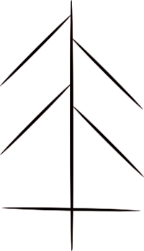
\includegraphics[height=5.5cm]{setup/Pictures/Nagerune.png}
    \caption{Nagerune}
\end{figure}

\textbf{Elementrune}\\
Denne rune besidder alle elementernes kræfter. Hvordan den er opstået ved ingen præcist, men dværgene har dog legender, der fortæller om et uhyre, som levede i fortiden som skabte denne rune. Elementrunens kræfter kan være både offensive og defensive.\\
\begin{figure}[H]
    \centering
    
\includegraphics[height=5.5cm]{setup/Pictures/Elementrune.png}
    \caption{Elementrune}
\end{figure}

\textbf{Jernrune}\\
Denne rune er skabt til beskyttelse. Ifølge legenden blev den skabt af thanen Altika, som levede generationen efter Even Ûhr Krezz. Til tider er denne rune også kendt for at have
helbredende egenskaber.
\begin{figure}[H]
    \centering
    
\includegraphics[height=5.5cm]{setup/Pictures/Jernrune.png}
    \caption{Jernrune}
\end{figure}

\textbf{Dragerune}\\
Den nyeste rune, som først lige er blevet magtfuld. Med ophøjelsen af Esselia og dragernes Opvågning, har denne rune nu fået ny magt, som forstyrrer balancen.\\
\begin{figure}[H]
    \centering
    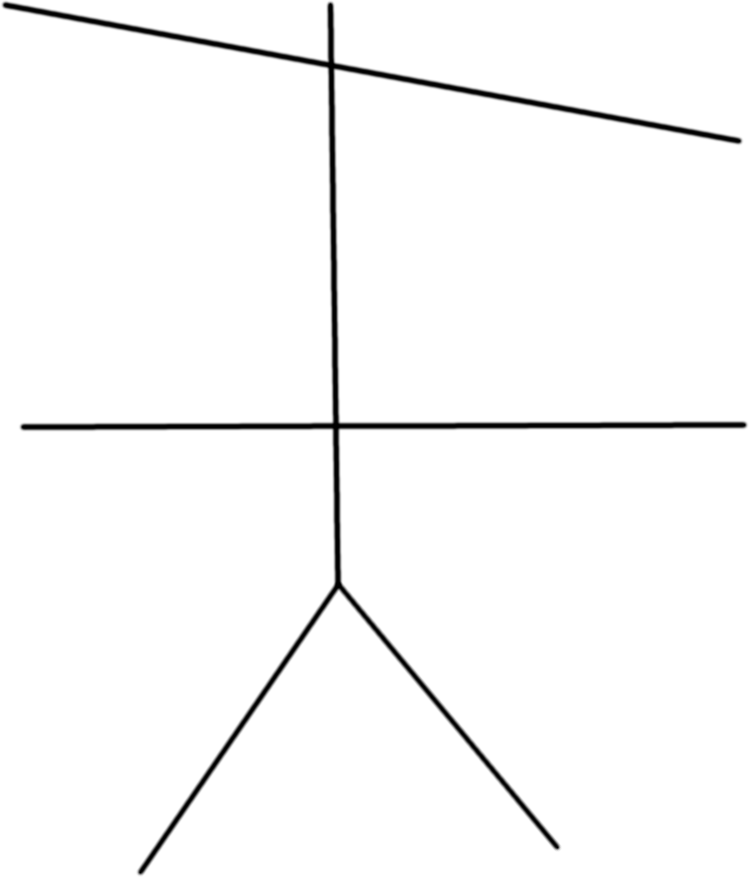
\includegraphics[height=5.5cm]{setup/Pictures/Dragerune.png}
    \caption{Dragerune}
\end{figure}

\begin{runeskjold*}[Drageskind]
\textbf{Effekt:} Du tager kun halvt så meget skade fra magier. (rundet op)\\
\textbf{Ingredienser:} 3 Elementruner, 3 Drageruner, 2 Jernruner.
\end{runeskjold*}

\begin{runeskjold*}[Essalias beskyttelse]
\textbf{Effekt:} Du får dobbelt så meget liv når du bliver helbredt.\\
\textbf{Ingredienser:} : 1 Elementrune, 1 Dragerune.
\end{runeskjold*}

\begin{runeskjold*}[Krigerens Skjold]
\textbf{Effekt:} Dette skjold giver dig 1 RP på samme måde som en normal rustningsdel vil. Det ekstra RP fra dit skjold vil altid være det første du mister; dette ekstra RP mistes kun når du selv rammes og ikke når nogen slår på skjoldet. Dette RP kan repareres som normalt hos en smed.\\
\textbf{Ingredienser:} : 1 Jernrune.
\end{runeskjold*}

\begin{runeskjold*}[Magiens Bane]
\textbf{Effekt:} Dette runeskjold gør bæreren i stand til 2 gange per døgn, at modstå en valgfri magi som rammer spilleren. Når spilleren rammes af en magi, de vil beskyttes imod, skal de udtale kommandoen: ”Magiens Bane – immun!”\\
\textbf{Ingredienser:} 4 Jern, 2 Jernruner, 2 Elementruner, 1 Dragerune.
\end{runeskjold*}

\begin{runevåben*}[Armens styrke]
\textbf{Effekt:} Bæreren af dette våben vil modtage 5 ekstra NK så længe de har våbenet på sig.\\
\textbf{Ingredienser:} 1 Nagerune
\end{runevåben*}

\begin{runevåben*}[Heksejægeren]
\textbf{Effekt:} En gang per døgn kan du ophæve en magi, hvis du rammer en person eller barriere med dette våben. Du kan ikke ophæve magiske genstande, såsom talismaner med dette våben.\\
\textbf{Ingredienser:} 1 Jern, 1 Sjælestøv, 1 Nagerune, 1 Jernrune, 1 Elementrune, 1 Dragerune.
\end{runevåben*}

\begin{runevåben*}[Kellwans Klinge]
\textbf{Effekt:} Dette våben giver permanent hellig skade. Dette skal som normalt markeres med et grønt bånd. (For optimal effekt kan dette også siges ved slag på fjender, hvor hellig skade kan have effekt.)\\
\textbf{Ingredienser:} 1 Nagerrune, 1 Elementrune.
\end{runevåben*}

\begin{runevåben*}[Livets Le]
\textbf{Effekt:} Når du dræber en person med dette våben vil du genvinde 1 mistet LP. Du kan ikke gå over din maksimale LP ved brug af dette våben.\\
\textbf{Ingredienser:} 1 Flagermuse gødning, 1 Elementrune, 2 Nagerruner, 1 Dragerune
\end{runevåben*}

\begin{runevåben*}[Magerens Mareridt]
Dette våben har ingen effekt i kamp. Det kan bruges til tortur, hvor den vil syge vilje og fokus fra ethvert offer. Tortureres en person med mana i kroppen, vil de miste mana i stedet for LP, med samme interval på 1 mana per minut. Offerets mana kan først genvindes 1 time efter torturen er afsluttet. Har offeret ingen mana (tilbage) i kroppen, vil de miste LP som ved normal tortur.
Note: Denne rune genstand tæller ikke mod det samlet antal rune genstande du må have på dig. Denne rune kan sættes på alle torturinstrumenter.\\
\textbf{Ingredienser:} 1 Nagerrune, 1 Enhjørningeblod.
\end{runevåben*}

\begin{runerustning*}[Dragens Rustning]
\textbf{Effekt:} 2 gange pr. scenarie kan du ved at berøre nogen bruge kommandoen: ”Drageild – 6 hellig skade”. Du vælger selv hvornår du bruger kommandoen.\\
\textbf{Ingredienser:} 4 Sulfur, 2 Dragerune, 2 Elementrune, 1 Ildgræs.
\end{runerustning*}

\begin{runerustning*}[Gudernes Rustning]
\textbf{Effekt:} Negative magier påvirker dig nu kun halvt så lang tid (rundet op.)\\
\textbf{Ingredienser:} 3 Drageruner, 1 Elementrune.
\end{runerustning*}

\begin{runerustning*}[Hærførens Rustning]
\textbf{Effekt:} Denne rustning giver dig 3 ekstra RP. Disse RP fungerer på samme måde som de normale RP du får fra en normal rustning. De ekstra RP vil altid være det første, du mister og de sidste der, bliver repareret.\\
\textbf{Ingredienser:} 4 Jern, 3 Jernruner.
\end{runerustning*}

\begin{runerustning*}[Jordens Rustning]
\textbf{Effekt:} Du bliver immun overfor alle vælte effekter\\
\textbf{Ingredienser:} 2 Jernruner, 2 Elementruner, 1 Flagermuse gødning.
\end{runerustning*}

\begin{runerustning*}[Krigerens Rustning]
\textbf{Effekt:} Denne rustning giver dig 2 ekstra RP. Disse RP fungerer på samme måde som de normale RP du får fra en normal rustning. De ekstra RP vil altid være det første, du mister og de sidste der, bliver repareret.\\
\textbf{Ingredienser:} 2 jern, 1 Jernrune.
\end{runerustning*}

\begin{runerustning*}[Samaritanernes Rustning]
\textbf{Effekt:} Hvis du går på 0 LP mens du bærer denne rustning, vil du automatisk genvinde alle dine naturlige LP 10 minutter efter du vågner; dvs. når du igen er kampdygtig ifølge dødsreglerne, som findes i det almindelige regelsæt.\\
\textbf{Ingredienser:} 1 Jernrune, 1 Enhjørningeblod.
\end{runerustning*}

\begin{runerustning*}[Thanens Rustning]
\textbf{Effekt:} Denne rustning reparerer alt din udrustning på mystisk vis. Dette betyder, at du genvinder 1 RP pr. 2. minut når du bærer rustningen og er ved bevidsthed. Du kan ikke genvinde mere RP end du normalt får for din rustning.\\
\textbf{Ingredienser:} 1 Jernrune, 1 Elementrune.
\end{runerustning*}


\end{document}